% Options for packages loaded elsewhere
\PassOptionsToPackage{unicode}{hyperref}
\PassOptionsToPackage{hyphens}{url}
%
\documentclass[
]{article}
\usepackage{amsmath,amssymb}
\usepackage{lmodern}
\usepackage{iftex}
\ifPDFTeX
  \usepackage[T1]{fontenc}
  \usepackage[utf8]{inputenc}
  \usepackage{textcomp} % provide euro and other symbols
\else % if luatex or xetex
  \usepackage{unicode-math}
  \defaultfontfeatures{Scale=MatchLowercase}
  \defaultfontfeatures[\rmfamily]{Ligatures=TeX,Scale=1}
\fi
% Use upquote if available, for straight quotes in verbatim environments
\IfFileExists{upquote.sty}{\usepackage{upquote}}{}
\IfFileExists{microtype.sty}{% use microtype if available
  \usepackage[]{microtype}
  \UseMicrotypeSet[protrusion]{basicmath} % disable protrusion for tt fonts
}{}
\makeatletter
\@ifundefined{KOMAClassName}{% if non-KOMA class
  \IfFileExists{parskip.sty}{%
    \usepackage{parskip}
  }{% else
    \setlength{\parindent}{0pt}
    \setlength{\parskip}{6pt plus 2pt minus 1pt}}
}{% if KOMA class
  \KOMAoptions{parskip=half}}
\makeatother
\usepackage{xcolor}
\usepackage[margin=1in]{geometry}
\usepackage{color}
\usepackage{fancyvrb}
\newcommand{\VerbBar}{|}
\newcommand{\VERB}{\Verb[commandchars=\\\{\}]}
\DefineVerbatimEnvironment{Highlighting}{Verbatim}{commandchars=\\\{\}}
% Add ',fontsize=\small' for more characters per line
\usepackage{framed}
\definecolor{shadecolor}{RGB}{248,248,248}
\newenvironment{Shaded}{\begin{snugshade}}{\end{snugshade}}
\newcommand{\AlertTok}[1]{\textcolor[rgb]{0.94,0.16,0.16}{#1}}
\newcommand{\AnnotationTok}[1]{\textcolor[rgb]{0.56,0.35,0.01}{\textbf{\textit{#1}}}}
\newcommand{\AttributeTok}[1]{\textcolor[rgb]{0.77,0.63,0.00}{#1}}
\newcommand{\BaseNTok}[1]{\textcolor[rgb]{0.00,0.00,0.81}{#1}}
\newcommand{\BuiltInTok}[1]{#1}
\newcommand{\CharTok}[1]{\textcolor[rgb]{0.31,0.60,0.02}{#1}}
\newcommand{\CommentTok}[1]{\textcolor[rgb]{0.56,0.35,0.01}{\textit{#1}}}
\newcommand{\CommentVarTok}[1]{\textcolor[rgb]{0.56,0.35,0.01}{\textbf{\textit{#1}}}}
\newcommand{\ConstantTok}[1]{\textcolor[rgb]{0.00,0.00,0.00}{#1}}
\newcommand{\ControlFlowTok}[1]{\textcolor[rgb]{0.13,0.29,0.53}{\textbf{#1}}}
\newcommand{\DataTypeTok}[1]{\textcolor[rgb]{0.13,0.29,0.53}{#1}}
\newcommand{\DecValTok}[1]{\textcolor[rgb]{0.00,0.00,0.81}{#1}}
\newcommand{\DocumentationTok}[1]{\textcolor[rgb]{0.56,0.35,0.01}{\textbf{\textit{#1}}}}
\newcommand{\ErrorTok}[1]{\textcolor[rgb]{0.64,0.00,0.00}{\textbf{#1}}}
\newcommand{\ExtensionTok}[1]{#1}
\newcommand{\FloatTok}[1]{\textcolor[rgb]{0.00,0.00,0.81}{#1}}
\newcommand{\FunctionTok}[1]{\textcolor[rgb]{0.00,0.00,0.00}{#1}}
\newcommand{\ImportTok}[1]{#1}
\newcommand{\InformationTok}[1]{\textcolor[rgb]{0.56,0.35,0.01}{\textbf{\textit{#1}}}}
\newcommand{\KeywordTok}[1]{\textcolor[rgb]{0.13,0.29,0.53}{\textbf{#1}}}
\newcommand{\NormalTok}[1]{#1}
\newcommand{\OperatorTok}[1]{\textcolor[rgb]{0.81,0.36,0.00}{\textbf{#1}}}
\newcommand{\OtherTok}[1]{\textcolor[rgb]{0.56,0.35,0.01}{#1}}
\newcommand{\PreprocessorTok}[1]{\textcolor[rgb]{0.56,0.35,0.01}{\textit{#1}}}
\newcommand{\RegionMarkerTok}[1]{#1}
\newcommand{\SpecialCharTok}[1]{\textcolor[rgb]{0.00,0.00,0.00}{#1}}
\newcommand{\SpecialStringTok}[1]{\textcolor[rgb]{0.31,0.60,0.02}{#1}}
\newcommand{\StringTok}[1]{\textcolor[rgb]{0.31,0.60,0.02}{#1}}
\newcommand{\VariableTok}[1]{\textcolor[rgb]{0.00,0.00,0.00}{#1}}
\newcommand{\VerbatimStringTok}[1]{\textcolor[rgb]{0.31,0.60,0.02}{#1}}
\newcommand{\WarningTok}[1]{\textcolor[rgb]{0.56,0.35,0.01}{\textbf{\textit{#1}}}}
\usepackage{longtable,booktabs,array}
\usepackage{calc} % for calculating minipage widths
% Correct order of tables after \paragraph or \subparagraph
\usepackage{etoolbox}
\makeatletter
\patchcmd\longtable{\par}{\if@noskipsec\mbox{}\fi\par}{}{}
\makeatother
% Allow footnotes in longtable head/foot
\IfFileExists{footnotehyper.sty}{\usepackage{footnotehyper}}{\usepackage{footnote}}
\makesavenoteenv{longtable}
\usepackage{graphicx}
\makeatletter
\def\maxwidth{\ifdim\Gin@nat@width>\linewidth\linewidth\else\Gin@nat@width\fi}
\def\maxheight{\ifdim\Gin@nat@height>\textheight\textheight\else\Gin@nat@height\fi}
\makeatother
% Scale images if necessary, so that they will not overflow the page
% margins by default, and it is still possible to overwrite the defaults
% using explicit options in \includegraphics[width, height, ...]{}
\setkeys{Gin}{width=\maxwidth,height=\maxheight,keepaspectratio}
% Set default figure placement to htbp
\makeatletter
\def\fps@figure{htbp}
\makeatother
\setlength{\emergencystretch}{3em} % prevent overfull lines
\providecommand{\tightlist}{%
  \setlength{\itemsep}{0pt}\setlength{\parskip}{0pt}}
\setcounter{secnumdepth}{5}
\usepackage{booktabs}
\usepackage{longtable}
\usepackage{array}
\usepackage{multirow}
\usepackage{wrapfig}
\usepackage{float}
\usepackage{colortbl}
\usepackage{pdflscape}
\usepackage{tabu}
\usepackage{threeparttable}
\usepackage{threeparttablex}
\usepackage[normalem]{ulem}
\usepackage{makecell}
\usepackage{xcolor}
\ifLuaTeX
  \usepackage{selnolig}  % disable illegal ligatures
\fi
\IfFileExists{bookmark.sty}{\usepackage{bookmark}}{\usepackage{hyperref}}
\IfFileExists{xurl.sty}{\usepackage{xurl}}{} % add URL line breaks if available
\urlstyle{same} % disable monospaced font for URLs
\hypersetup{
  pdftitle={Projeto da Pós Graduação, disciplina Estatística para Cientista de Dados.},
  pdfauthor={Antonio Vieira dos Santos Neto - Cpf 077.523.948-82},
  hidelinks,
  pdfcreator={LaTeX via pandoc}}

\title{Projeto da Pós Graduação, disciplina Estatística para Cientista de Dados.}
\author{Antonio Vieira dos Santos Neto - Cpf 077.523.948-82}
\date{2023-03-10}

\begin{document}
\maketitle

{
\setcounter{tocdepth}{2}
\tableofcontents
}
\hypertarget{introduuxe7uxe3o}{%
\subsection{Introdução}\label{introduuxe7uxe3o}}

O presente projeto visa demonstrar os conhecimentos nos fundamentos básicos na utilização da linguagem ``R'', bem como, nos conhecimentos de Estatística.

Neste documento, segue o passo a passo, onde são demonstrados os conhecimentos adquiridos na disciplina.

\hypertarget{objetivo-do-projeto}{%
\subsection{Objetivo do Projeto}\label{objetivo-do-projeto}}

Demonstrar os conhecimentos adquiridos na disciplina ``Estatística para Cientista de Dados'', sendo que , através do uso da Linguagem ``R'', serão feitas diversas análises em uma ``Base de evolução de registro de ocorrências do Instituto de Segurança Pública do Rio de Janeiro''.

\hypertarget{preparando-o-ambiente-de-anuxe1lise}{%
\subsection{Preparando o ambiente de análise}\label{preparando-o-ambiente-de-anuxe1lise}}

Para a criação do ambiente de trabalho foram adotados os seguinte passos :

\begin{itemize}
\item
  1-Instalação da linguagem ``R'' na máquina do aluno.
\item
  2-Instalação do Studio ``R'' na máquina do aluno.
\item
  3-Instalação do ``GIT'' na máquina do aluno. Esta aplicação permite o controle dos versionamentos dos aplicações desenvolvidas.
\item
  4-Configuração na nuvem do ``GITHUB, criando um repositório''WORK'', para arquivo das aplicações desenvolvidas, bem como, controle do versionamento destas.
\item
  Atenção:
\item
  1 - As evidências da configuração do ambiente, segue no documento ``Antonio Vieria dos Santos Neto\_Estatisticas para Cientista de Dados\_evidencias.pdf''
\item
  2 - O caminho para o Github do aluno e´: \url{https://github.com/avsneto2/work.git}
\item
  3- Os arquivos do projeto se encontram na branch : Projeto\_Estatistica\_1
\end{itemize}

\hypertarget{importando-bibliotecas-necessuxe1rias-ao-desenvolvimento.--}{%
\paragraph{Importando bibliotecas necessárias ao desenvolvimento. -}\label{importando-bibliotecas-necessuxe1rias-ao-desenvolvimento.--}}

Para suporte no tratamento da base de dados, foram instaladas as bibliotecas a seguir a partir do comando ``install.packages''.

\begin{itemize}
\item
  install.packages(``tidyverse'') - Pacote de ferramentas que tem por objetivo manipulação, exploração e visualização de dados.
\item
  install.packages(``data.table'') - Pacote que também tem a função de manipular dados, porém, em algumas situações, permite o tratamento de dados com maior velocidade
\item
  install.packages(``rvest'') - Uma das funções do Pacote ``rvest'' e permitir a leitura de dados a partir de código html, dessa forma o ``R'' poderá mapear e navegar pela arvore do html.
\item
  install.packages(``robotstxt'') - Este pacote fornece funcoes para baixar e analisar arquivos `robots.txt'.
\item
  install.packages(``knitr'') - Este pacote tem a funcao de gerar relatorios dinamicos com R.
\item
  instal.packages (``dlookr'') - Este pacote informações estatísticas sobre dados como visualização, valores ausentes, discrepantes e valores exclusivos e negativos, com o objetivo de entender a distribuição e qualidade dos dados.
\item
  instal.packages (``readxl'') - Este pacote permite a leitura de arquivos excel.
\item
  instal.packages (``summarytools'') - Este pacote permite a análise de dados, como a frequencia de uma determinada variavel;
\item
  instal.packages (``ggplot2'') - Este pacote permite o desenvolvimento de graficos;
\item
  instal.packages (``fitdistrplus'') - Pacote com várias funções para ajudar no ajuste de uma distribuição paramétrica a dados não censurados ou censurados.
\end{itemize}

\begin{Shaded}
\begin{Highlighting}[]
\FunctionTok{library}\NormalTok{(tidyverse)}
\end{Highlighting}
\end{Shaded}

\begin{verbatim}
## -- Attaching packages --------------------------------------- tidyverse 1.3.2 --
## v ggplot2 3.4.1     v purrr   1.0.1
## v tibble  3.1.8     v dplyr   1.1.0
## v tidyr   1.3.0     v stringr 1.5.0
## v readr   2.1.4     v forcats 1.0.0
## -- Conflicts ------------------------------------------ tidyverse_conflicts() --
## x dplyr::filter() masks stats::filter()
## x dplyr::lag()    masks stats::lag()
\end{verbatim}

\begin{Shaded}
\begin{Highlighting}[]
\FunctionTok{library}\NormalTok{(rvest)}
\end{Highlighting}
\end{Shaded}

\begin{verbatim}
## 
## Attaching package: 'rvest'
## 
## The following object is masked from 'package:readr':
## 
##     guess_encoding
\end{verbatim}

\begin{Shaded}
\begin{Highlighting}[]
\FunctionTok{library}\NormalTok{(data.table)}
\end{Highlighting}
\end{Shaded}

\begin{verbatim}
## 
## Attaching package: 'data.table'
## 
## The following objects are masked from 'package:dplyr':
## 
##     between, first, last
## 
## The following object is masked from 'package:purrr':
## 
##     transpose
\end{verbatim}

\begin{Shaded}
\begin{Highlighting}[]
\FunctionTok{library}\NormalTok{(robotstxt)}
\FunctionTok{library}\NormalTok{(knitr)}
\FunctionTok{library}\NormalTok{(dlookr)}
\end{Highlighting}
\end{Shaded}

\begin{verbatim}
## Warning in !is.null(rmarkdown::metadata$output) && rmarkdown::metadata$output
## %in% : 'length(x) = 2 > 1' in coercion to 'logical(1)'
\end{verbatim}

\begin{verbatim}
## 
## Attaching package: 'dlookr'
## 
## The following object is masked from 'package:tidyr':
## 
##     extract
## 
## The following object is masked from 'package:base':
## 
##     transform
\end{verbatim}

\begin{Shaded}
\begin{Highlighting}[]
\FunctionTok{library}\NormalTok{(readxl)}
\FunctionTok{library}\NormalTok{(summarytools)}
\end{Highlighting}
\end{Shaded}

\begin{verbatim}
## 
## Attaching package: 'summarytools'
## 
## The following object is masked from 'package:tibble':
## 
##     view
\end{verbatim}

\begin{Shaded}
\begin{Highlighting}[]
\FunctionTok{library}\NormalTok{(ggplot2)}
\FunctionTok{library}\NormalTok{(fitdistrplus)}
\end{Highlighting}
\end{Shaded}

\begin{verbatim}
## Carregando pacotes exigidos: MASS
## 
## Attaching package: 'MASS'
## 
## The following object is masked from 'package:dplyr':
## 
##     select
## 
## Carregando pacotes exigidos: survival
\end{verbatim}

\begin{Shaded}
\begin{Highlighting}[]
\FunctionTok{library}\NormalTok{(readr)}
\end{Highlighting}
\end{Shaded}

\hypertarget{definindo-o-diretuxf3rio-de-trabalho-para-o-projeto}{%
\paragraph{Definindo o diretório de trabalho para o projeto}\label{definindo-o-diretuxf3rio-de-trabalho-para-o-projeto}}

Posteriomente, vamos trocar o diretório de referência para o trabalho, mas não vamos deixar essa informação pública para o usuário.

\begin{verbatim}
## [1] "E:/DADOS/VIEIRA/POS GRADUACAO/INFINET/CURSO/WORK_Trabalho/work"
\end{verbatim}

\hypertarget{importando-dados--}{%
\paragraph{Importando dados -}\label{importando-dados--}}

A partir da definição do ambiente, o arquivo ``BaseDPEvolucaoMensalCisp.csv'', contendo a base de evolução de registro de ocorrencias do Instituto de Segurança Publica do Rio de Janeiro, será importado utilizando a biblioteca rvest, para ler o arquivo ``CSV.

\begin{Shaded}
\begin{Highlighting}[]
\DocumentationTok{\#\# Bevolucao.tbl \textless{}{-} readr::read\_csv2("BaseDPEvolucaoMensalCisp.csv")}
\NormalTok{Bevolucao.tbl }\OtherTok{\textless{}{-}}\NormalTok{ readr}\SpecialCharTok{::}\FunctionTok{read\_csv2}\NormalTok{(}\StringTok{"BaseDPEvolucaoMensalCisp.csv"}\NormalTok{, }\AttributeTok{locale=}\FunctionTok{locale}\NormalTok{(}\AttributeTok{encoding=}\StringTok{"latin1"}\NormalTok{))}
\end{Highlighting}
\end{Shaded}

\begin{verbatim}
## i Using "','" as decimal and "'.'" as grouping mark. Use `read_delim()` for more control.
\end{verbatim}

\begin{verbatim}
## Rows: 32245 Columns: 63
## -- Column specification --------------------------------------------------------
## Delimiter: ";"
## chr  (3): mes_ano, munic, Regiao
## dbl (60): CISP, mes, ano, AISP, RISP, mcirc, hom_doloso, lesao_corp_morte, l...
## 
## i Use `spec()` to retrieve the full column specification for this data.
## i Specify the column types or set `show_col_types = FALSE` to quiet this message.
\end{verbatim}

\begin{Shaded}
\begin{Highlighting}[]
\FunctionTok{kable}\NormalTok{(}\FunctionTok{head}\NormalTok{(Bevolucao.tbl))}
\end{Highlighting}
\end{Shaded}

\begin{tabular}{r|r|r|l|r|r|l|r|l|r|r|r|r|r|r|r|r|r|r|r|r|r|r|r|r|r|r|r|r|r|r|r|r|r|r|r|r|r|r|r|r|r|r|r|r|r|r|r|r|r|r|r|r|r|r|r|r|r|r|r|r|r|r}
\hline
CISP & mes & ano & mes\_ano & AISP & RISP & munic & mcirc & Regiao & hom\_doloso & lesao\_corp\_morte & latrocinio & cvli & hom\_por\_interv\_policial & letalidade\_violenta & tentat\_hom & lesao\_corp\_dolosa & estupro & hom\_culposo & lesao\_corp\_culposa & roubo\_transeunte & roubo\_celular & roubo\_em\_coletivo & roubo\_rua & roubo\_veiculo & roubo\_carga & roubo\_comercio & roubo\_residencia & roubo\_banco & roubo\_cx\_eletronico & roubo\_conducao\_saque & roubo\_apos\_saque & roubo\_bicicleta & outros\_roubos & total\_roubos & furto\_veiculos & furto\_transeunte & furto\_coletivo & furto\_celular & furto\_bicicleta & outros\_furtos & total\_furtos & sequestro & extorsao & sequestro\_relampago & estelionato & apreensao\_drogas & posse\_drogas & trafico\_drogas & apreensao\_drogas\_sem\_autor & recuperacao\_veiculos & apf & aaapai & cmp & cmba & ameaca & pessoas\_desaparecidas & encontro\_cadaver & encontro\_ossada & pol\_militares\_mortos\_serv & pol\_civis\_mortos\_serv & registro\_ocorrencias & fase\\
\hline
1 & 1 & 2003 & 2003m01 & 5 & 1 & Rio de Janeiro & 3304557 & Capital & 0 & 0 & 0 & 0 & 0 & 0 & 1 & 40 & 0 & 1 & 15 & 26 & 32 & 8 & 66 & 5 & 1 & 14 & 0 & 0 & 0 & 0 & 10 & NA & 4 & 100 & 12 & 30 & 0 & 37 & NA & 90 & 169 & 0 & 1 & 0 & 69 & 1 & NA & NA & NA & 5 & NA & NA & NA & NA & 21 & 2 & 0 & 0 & 0 & 0 & 578 & 3\\
\hline
4 & 1 & 2003 & 2003m01 & 5 & 1 & Rio de Janeiro & 3304557 & Capital & 3 & 0 & 0 & 3 & 0 & 3 & 0 & 47 & 1 & 4 & 35 & 25 & 14 & 12 & 51 & 9 & 1 & 5 & 0 & 0 & 1 & 1 & 3 & NA & 11 & 82 & 9 & 42 & 5 & 23 & NA & 36 & 115 & 0 & 1 & 0 & 1 & 35 & NA & NA & NA & 7 & NA & NA & NA & NA & 15 & 6 & 0 & 1 & 0 & 0 & 441 & 3\\
\hline
5 & 1 & 2003 & 2003m01 & 5 & 1 & Rio de Janeiro & 3304557 & Capital & 3 & 0 & 0 & 3 & 0 & 3 & 1 & 73 & 2 & 1 & 19 & 26 & 34 & 4 & 64 & 11 & 5 & 10 & 1 & 2 & 0 & 2 & 4 & NA & 24 & 123 & 28 & 42 & 2 & 47 & NA & 97 & 216 & 0 & 0 & 0 & 37 & 4 & NA & NA & NA & 10 & NA & NA & NA & NA & 47 & 2 & 1 & 0 & 0 & 0 & 637 & 3\\
\hline
6 & 1 & 2003 & 2003m01 & 1 & 1 & Rio de Janeiro & 3304557 & Capital & 6 & 0 & 0 & 6 & 0 & 6 & 2 & 43 & 2 & 1 & 20 & 14 & 20 & 22 & 56 & 27 & 6 & 10 & 0 & 0 & 0 & 0 & 6 & NA & 38 & 143 & 17 & 4 & 0 & 8 & NA & 61 & 90 & 0 & 0 & 0 & 8 & 20 & NA & NA & NA & 77 & NA & NA & NA & NA & 26 & 2 & 1 & 0 & 0 & 0 & 473 & 3\\
\hline
7 & 1 & 2003 & 2003m01 & 1 & 1 & Rio de Janeiro & 3304557 & Capital & 4 & 0 & 0 & 4 & 0 & 4 & 2 & 18 & 2 & 0 & 2 & 4 & 1 & 0 & 5 & 23 & 1 & 0 & 2 & 0 & 0 & 0 & 1 & NA & 23 & 55 & 12 & 1 & 0 & 1 & NA & 21 & 35 & 0 & 0 & 0 & 4 & 3 & NA & NA & NA & 9 & NA & NA & NA & NA & 10 & 1 & 3 & 0 & 0 & 0 & 147 & 3\\
\hline
9 & 1 & 2003 & 2003m01 & 2 & 1 & Rio de Janeiro & 3304557 & Capital & 1 & 1 & 0 & 2 & 0 & 2 & 3 & 44 & 0 & 0 & 15 & 18 & 16 & 10 & 44 & 30 & 0 & 4 & 3 & 0 & 0 & 0 & 2 & NA & 41 & 124 & 87 & 40 & 1 & 16 & NA & 124 & 268 & 0 & 0 & 0 & 20 & 11 & NA & NA & NA & 20 & NA & NA & NA & NA & 36 & 3 & 0 & 0 & 0 & 0 & 554 & 3\\
\hline
\end{tabular}

\hypertarget{selecionando-dados--}{%
\paragraph{Selecionando dados -}\label{selecionando-dados--}}

Uma vez que os dados foram importados, faremos a seleção das colunas importantes para a análise. Dessa forma, serão selecionados os dados referentes as ocorrencias relacionadas ao evento de apreensão de drogas versus roubos.

\begin{Shaded}
\begin{Highlighting}[]
\NormalTok{Bevolucao.roubos.tbl }\OtherTok{\textless{}{-}}\NormalTok{ Bevolucao.tbl }\SpecialCharTok{\%\textgreater{}\%}\NormalTok{ dplyr}\SpecialCharTok{::}\FunctionTok{select}\NormalTok{(CISP,ano,mes\_ano,munic,Regiao,apreensao\_drogas, roubo\_transeunte,roubo\_celular,roubo\_residencia, roubo\_rua)}
\FunctionTok{kable}\NormalTok{(}\FunctionTok{head}\NormalTok{(Bevolucao.roubos.tbl))}
\end{Highlighting}
\end{Shaded}

\begin{tabular}{r|r|l|l|l|r|r|r|r|r}
\hline
CISP & ano & mes\_ano & munic & Regiao & apreensao\_drogas & roubo\_transeunte & roubo\_celular & roubo\_residencia & roubo\_rua\\
\hline
1 & 2003 & 2003m01 & Rio de Janeiro & Capital & 1 & 26 & 32 & 0 & 66\\
\hline
4 & 2003 & 2003m01 & Rio de Janeiro & Capital & 35 & 25 & 14 & 0 & 51\\
\hline
5 & 2003 & 2003m01 & Rio de Janeiro & Capital & 4 & 26 & 34 & 1 & 64\\
\hline
6 & 2003 & 2003m01 & Rio de Janeiro & Capital & 20 & 14 & 20 & 0 & 56\\
\hline
7 & 2003 & 2003m01 & Rio de Janeiro & Capital & 3 & 4 & 1 & 2 & 5\\
\hline
9 & 2003 & 2003m01 & Rio de Janeiro & Capital & 11 & 18 & 16 & 3 & 44\\
\hline
\end{tabular}

\hypertarget{selecionando-os-movimentos-referentes-aos-truxeas-uxfaltimos-anos--}{%
\paragraph{Selecionando os movimentos referentes aos três últimos anos -}\label{selecionando-os-movimentos-referentes-aos-truxeas-uxfaltimos-anos--}}

Com base na coluna ano, selecionar o movimento dos três últimos anos.

\begin{Shaded}
\begin{Highlighting}[]
\NormalTok{Bevolucao.roubos.f1.tbl}\OtherTok{=}\NormalTok{Bevolucao.roubos.tbl }\SpecialCharTok{\%\textgreater{}\%}\NormalTok{ dplyr}\SpecialCharTok{::}\FunctionTok{filter}\NormalTok{ (ano }\SpecialCharTok{==}\StringTok{\textquotesingle{}2022\textquotesingle{}}\SpecialCharTok{|}\NormalTok{ ano }\SpecialCharTok{==}\StringTok{\textquotesingle{}2021\textquotesingle{}} \SpecialCharTok{|}\NormalTok{ ano }\SpecialCharTok{==}\StringTok{\textquotesingle{}2020\textquotesingle{}}\NormalTok{)}
\FunctionTok{kable}\NormalTok{(}\FunctionTok{head}\NormalTok{(Bevolucao.roubos.f1.tbl))}
\end{Highlighting}
\end{Shaded}

\begin{tabular}{r|r|l|l|l|r|r|r|r|r}
\hline
CISP & ano & mes\_ano & munic & Regiao & apreensao\_drogas & roubo\_transeunte & roubo\_celular & roubo\_residencia & roubo\_rua\\
\hline
1 & 2020 & 2020m01 & Rio de Janeiro & Capital & 2 & 62 & 32 & 0 & 107\\
\hline
4 & 2020 & 2020m01 & Rio de Janeiro & Capital & 7 & 59 & 19 & 1 & 99\\
\hline
5 & 2020 & 2020m01 & Rio de Janeiro & Capital & 13 & 130 & 36 & 0 & 179\\
\hline
6 & 2020 & 2020m01 & Rio de Janeiro & Capital & 3 & 63 & 15 & 0 & 99\\
\hline
7 & 2020 & 2020m01 & Rio de Janeiro & Capital & 1 & 27 & 2 & 0 & 35\\
\hline
9 & 2020 & 2020m01 & Rio de Janeiro & Capital & 6 & 69 & 27 & 0 & 103\\
\hline
\end{tabular}

\hypertarget{agrupando-por-regiao-munic-ano-e-mesano.--}{%
\paragraph{Agrupando por regiao, munic, ano e mes/ano. -}\label{agrupando-por-regiao-munic-ano-e-mesano.--}}

Vamos agrupar os dados por regiao, municipio e ano,com o objetivo de entender o movimento das ocorrencias de roubo no periodo.

\begin{Shaded}
\begin{Highlighting}[]
\NormalTok{Bevolucao.roubos.f2.tbl }\OtherTok{\textless{}{-}}\NormalTok{ Bevolucao.roubos.f1.tbl }\SpecialCharTok{\%\textgreater{}\%}\NormalTok{ dplyr}\SpecialCharTok{::}\FunctionTok{group\_by}\NormalTok{(Regiao, munic, ano, mes\_ano) }\SpecialCharTok{\%\textgreater{}\%}\NormalTok{ dplyr}\SpecialCharTok{::}\FunctionTok{summarise}\NormalTok{(}\AttributeTok{roubo\_transeunte\_sum =} \FunctionTok{sum}\NormalTok{(roubo\_transeunte), }\AttributeTok{apreensao\_drogas\_sum =} \FunctionTok{sum}\NormalTok{(apreensao\_drogas),}\AttributeTok{roubo\_celular\_sum =} \FunctionTok{sum}\NormalTok{(roubo\_celular),}\AttributeTok{roubo\_residencia\_sum =} \FunctionTok{sum}\NormalTok{(roubo\_residencia),}\AttributeTok{roubo\_rua\_sum =}\FunctionTok{sum}\NormalTok{(roubo\_rua))}
\end{Highlighting}
\end{Shaded}

\begin{verbatim}
## `summarise()` has grouped output by 'Regiao', 'munic', 'ano'. You can override
## using the `.groups` argument.
\end{verbatim}

\begin{Shaded}
\begin{Highlighting}[]
\FunctionTok{kable}\NormalTok{(}\FunctionTok{head}\NormalTok{(Bevolucao.roubos.f2.tbl))}
\end{Highlighting}
\end{Shaded}

\begin{tabular}{l|l|r|l|r|r|r|r|r}
\hline
Regiao & munic & ano & mes\_ano & roubo\_transeunte\_sum & apreensao\_drogas\_sum & roubo\_celular\_sum & roubo\_residencia\_sum & roubo\_rua\_sum\\
\hline
Baixada Fluminense & Belford Roxo & 2020 & 2020m01 & 198 & 17 & 58 & 0 & 296\\
\hline
Baixada Fluminense & Belford Roxo & 2020 & 2020m02 & 165 & 19 & 62 & 1 & 295\\
\hline
Baixada Fluminense & Belford Roxo & 2020 & 2020m03 & 87 & 17 & 33 & 1 & 141\\
\hline
Baixada Fluminense & Belford Roxo & 2020 & 2020m04 & 50 & 11 & 23 & 0 & 81\\
\hline
Baixada Fluminense & Belford Roxo & 2020 & 2020m05 & 106 & 4 & 71 & 1 & 181\\
\hline
Baixada Fluminense & Belford Roxo & 2020 & 2020m06 & 112 & 2 & 72 & 0 & 205\\
\hline
\end{tabular}

\hypertarget{convertendo-dados-da-coluna-mes_ano--}{%
\paragraph{Convertendo dados da coluna ``mes\_ano'' -}\label{convertendo-dados-da-coluna-mes_ano--}}

Os dados da coluna ``mes\_ano'' encontram-se no formato ``aaaammm'' e deverão ser convertidos para o formato ``aaaa-mm''.

\begin{Shaded}
\begin{Highlighting}[]
\NormalTok{Bevolucao.roubos.f3.tbl }\OtherTok{\textless{}{-}}\NormalTok{Bevolucao.roubos.f2.tbl }\SpecialCharTok{\%\textgreater{}\%}\NormalTok{ dplyr}\SpecialCharTok{::}\FunctionTok{mutate}\NormalTok{(}\AttributeTok{mes\_ano =}\NormalTok{ stringr}\SpecialCharTok{::}\FunctionTok{str\_replace\_all}\NormalTok{(mes\_ano, }\StringTok{"}\SpecialCharTok{\textbackslash{}\textbackslash{}}\StringTok{m"}\NormalTok{, }\StringTok{"{-}"}\NormalTok{))}

\FunctionTok{kable}\NormalTok{(}\FunctionTok{head}\NormalTok{(Bevolucao.roubos.f3.tbl))}
\end{Highlighting}
\end{Shaded}

\begin{tabular}{l|l|r|l|r|r|r|r|r}
\hline
Regiao & munic & ano & mes\_ano & roubo\_transeunte\_sum & apreensao\_drogas\_sum & roubo\_celular\_sum & roubo\_residencia\_sum & roubo\_rua\_sum\\
\hline
Baixada Fluminense & Belford Roxo & 2020 & 2020-01 & 198 & 17 & 58 & 0 & 296\\
\hline
Baixada Fluminense & Belford Roxo & 2020 & 2020-02 & 165 & 19 & 62 & 1 & 295\\
\hline
Baixada Fluminense & Belford Roxo & 2020 & 2020-03 & 87 & 17 & 33 & 1 & 141\\
\hline
Baixada Fluminense & Belford Roxo & 2020 & 2020-04 & 50 & 11 & 23 & 0 & 81\\
\hline
Baixada Fluminense & Belford Roxo & 2020 & 2020-05 & 106 & 4 & 71 & 1 & 181\\
\hline
Baixada Fluminense & Belford Roxo & 2020 & 2020-06 & 112 & 2 & 72 & 0 & 205\\
\hline
\end{tabular}

\hypertarget{iniciando-a-analise-dos-dados}{%
\subsection{Iniciando a analise dos dados}\label{iniciando-a-analise-dos-dados}}

\hypertarget{identificando-os-tipos-de-variaveis--}{%
\paragraph{Identificando os tipos de variaveis -}\label{identificando-os-tipos-de-variaveis--}}

Para identificar os tipos de cada variável na base, vamos utilizar o pacote ``dlookr''e a função ``diagnose''.

\begin{Shaded}
\begin{Highlighting}[]
\NormalTok{Bevolucao.roubos.f3.tbl}\SpecialCharTok{\%\textgreater{}\%}\NormalTok{ dlookr}\SpecialCharTok{::}\FunctionTok{diagnose}\NormalTok{()}
\end{Highlighting}
\end{Shaded}

\begin{verbatim}
## # A tibble: 9 x 6
##   variables            types     missing_count missing_percent unique_~1 uniqu~2
##   <chr>                <chr>             <int>           <dbl>     <int>   <dbl>
## 1 Regiao               character             0               0         4 0.00136
## 2 munic                character             0               0        82 0.0278 
## 3 ano                  numeric               0               0         3 0.00102
## 4 mes_ano              character             0               0        36 0.0122 
## 5 roubo_transeunte_sum numeric               0               0       249 0.0843 
## 6 apreensao_drogas_sum numeric               0               0       141 0.0478 
## 7 roubo_celular_sum    numeric               0               0       145 0.0491 
## 8 roubo_residencia_sum numeric               0               0        34 0.0115 
## 9 roubo_rua_sum        numeric               0               0       311 0.105  
## # ... with abbreviated variable names 1: unique_count, 2: unique_rate
\end{verbatim}

Na tabela ``Bevolucao.roubos.f3.tbl'' é possivel identificar as variaveis do tipo QUALITATIVAS NOMINAIS que são:

\begin{itemize}
\tightlist
\item
  Regiao = Regiao
\item
  munic = Municipio
\item
  ano = ano relacionado ao registro das ocorrencias.
\item
  mes\_ano= mes e ano relacionado ao registro das ocorrencias
\end{itemize}

Na tabela ``Bevolucao.roubos.f3.tbl'' e possivel identificar as variaveis do tipo QUANTITATIVAS DISCRETAS que são:

\begin{itemize}
\tightlist
\item
  roubo\_transeunte\_sum
\item
  apreensao\_drogas\_sum
\item
  roubo\_celular\_sum
\item
  roubo\_residencia\_sum
\item
  roubo\_rua\_sum
\end{itemize}

\hypertarget{identicando-a-frequencia-de-variaveis}{%
\paragraph{Identicando a frequencia de variaveis}\label{identicando-a-frequencia-de-variaveis}}

Para o próximo passo será analisada a frequencia das variaveis, dessa forma identificando a região com maior incidencia de ocorrencias.

Dessa forma a base foi sumarizada pelas variaveis ``Ano(ano)'', ``Regiao(Regiao)'' e ``Municipio(munic)'', sendo que, para cada ano, foi verificada a frequencia da variavel ``Regiao''.

\begin{Shaded}
\begin{Highlighting}[]
\NormalTok{Bevolucao.roubos.f4.tbl }\OtherTok{\textless{}{-}}\NormalTok{ Bevolucao.roubos.f3.tbl }\SpecialCharTok{\%\textgreater{}\%}\NormalTok{ dplyr}\SpecialCharTok{::}\FunctionTok{group\_by}\NormalTok{(ano, Regiao, munic) }\SpecialCharTok{\%\textgreater{}\%}\NormalTok{ dplyr}\SpecialCharTok{::}\FunctionTok{select}\NormalTok{(Regiao,ano,roubo\_transeunte\_sum, apreensao\_drogas\_sum,roubo\_celular\_sum,roubo\_residencia\_sum,roubo\_rua\_sum) }\SpecialCharTok{\%\textgreater{}\%}\NormalTok{ dplyr}\SpecialCharTok{::}\FunctionTok{summarise}\NormalTok{(}\AttributeTok{roubo\_transeunte\_sum =} \FunctionTok{sum}\NormalTok{(roubo\_transeunte\_sum), }\AttributeTok{apreensao\_drogas\_sum =} \FunctionTok{sum}\NormalTok{(apreensao\_drogas\_sum),}\AttributeTok{roubo\_celular\_sum =} \FunctionTok{sum}\NormalTok{(roubo\_celular\_sum),}\AttributeTok{roubo\_residencia\_sum =} \FunctionTok{sum}\NormalTok{(roubo\_residencia\_sum),}\AttributeTok{roubo\_rua\_sum =} \FunctionTok{sum}\NormalTok{(roubo\_rua\_sum))}
\end{Highlighting}
\end{Shaded}

\begin{verbatim}
## Adding missing grouping variables: `munic`
## `summarise()` has grouped output by 'ano', 'Regiao'. You can override using the
## `.groups` argument.
\end{verbatim}

\begin{Shaded}
\begin{Highlighting}[]
\FunctionTok{kable}\NormalTok{(}\FunctionTok{head}\NormalTok{(Bevolucao.roubos.f4.tbl))}
\end{Highlighting}
\end{Shaded}

\begin{tabular}{r|l|l|r|r|r|r|r}
\hline
ano & Regiao & munic & roubo\_transeunte\_sum & apreensao\_drogas\_sum & roubo\_celular\_sum & roubo\_residencia\_sum & roubo\_rua\_sum\\
\hline
2020 & Baixada Fluminense & Belford Roxo & 1459 & 127 & 515 & 6 & 2256\\
\hline
2020 & Baixada Fluminense & Duque de Caxias & 3981 & 330 & 1038 & 33 & 5853\\
\hline
2020 & Baixada Fluminense & Guapimirim & 47 & 65 & 28 & 6 & 75\\
\hline
2020 & Baixada Fluminense & Itaguaí & 183 & 66 & 66 & 7 & 260\\
\hline
2020 & Baixada Fluminense & Japeri & 94 & 60 & 38 & 4 & 149\\
\hline
2020 & Baixada Fluminense & Magé & 335 & 159 & 151 & 9 & 501\\
\hline
\end{tabular}

\begin{itemize}
\item
  Frequencia da variavel : Regiao
\item
  Conclusão :
  O que se observa com base na analise de frequencia, é que a maior ocorrencia dos eventos de roubos e apreensao de drogas, em termos de quantidade de municipios, se da na REGIAO DO INTERIOR DO RIO DE JANEIRO, com 79.27\% (65 ocorrencias).
\end{itemize}

\begin{Shaded}
\begin{Highlighting}[]
\NormalTok{Bevolucao.roubos.f4.tbl }\SpecialCharTok{\%\textgreater{}\%}\NormalTok{ dplyr}\SpecialCharTok{::}\FunctionTok{group\_by}\NormalTok{(ano) }\SpecialCharTok{\%\textgreater{}\%}\NormalTok{ dplyr}\SpecialCharTok{::}\FunctionTok{select}\NormalTok{(Regiao) }\SpecialCharTok{\%\textgreater{}\%}\NormalTok{ summarytools}\SpecialCharTok{::}\FunctionTok{freq}\NormalTok{()}
\end{Highlighting}
\end{Shaded}

\begin{verbatim}
## Adding missing grouping variables: `ano`
\end{verbatim}

\begin{verbatim}
## Frequencies  
## Bevolucao.roubos.f4.tbl$Regiao  
## Type: Character  
## Group: ano = 2020  
## 
##                            Freq   % Valid   % Valid Cum.   % Total   % Total Cum.
## ------------------------ ------ --------- -------------- --------- --------------
##       Baixada Fluminense     13     15.85          15.85     15.85          15.85
##                  Capital      1      1.22          17.07      1.22          17.07
##           Grande Niterói      3      3.66          20.73      3.66          20.73
##                 Interior     65     79.27         100.00     79.27         100.00
##                     <NA>      0                               0.00         100.00
##                    Total     82    100.00         100.00    100.00         100.00
## 
## Group: ano = 2021  
## 
##                            Freq   % Valid   % Valid Cum.   % Total   % Total Cum.
## ------------------------ ------ --------- -------------- --------- --------------
##       Baixada Fluminense     13     15.85          15.85     15.85          15.85
##                  Capital      1      1.22          17.07      1.22          17.07
##           Grande Niterói      3      3.66          20.73      3.66          20.73
##                 Interior     65     79.27         100.00     79.27         100.00
##                     <NA>      0                               0.00         100.00
##                    Total     82    100.00         100.00    100.00         100.00
## 
## Group: ano = 2022  
## 
##                            Freq   % Valid   % Valid Cum.   % Total   % Total Cum.
## ------------------------ ------ --------- -------------- --------- --------------
##       Baixada Fluminense     13     15.85          15.85     15.85          15.85
##                  Capital      1      1.22          17.07      1.22          17.07
##           Grande Niterói      3      3.66          20.73      3.66          20.73
##                 Interior     65     79.27         100.00     79.27         100.00
##                     <NA>      0                               0.00         100.00
##                    Total     82    100.00         100.00    100.00         100.00
\end{verbatim}

\hypertarget{fazendo-analise-descritiva-e-de-histogramas-de-uma-variavel-quantitativa-discreta--}{%
\paragraph{Fazendo analise descritiva e de histogramas de uma variavel quantitativa discreta -}\label{fazendo-analise-descritiva-e-de-histogramas-de-uma-variavel-quantitativa-discreta--}}

Com base nas variaveis qualitativas (Ano e Regiao), foi feita uma análise considerando a centralidade dos dados para a variavel roubo\_transeunte\_sum e apreensao\_drogas\_sum, através da funcao descr do pacote summarytools (descr).

-Variavel roubo\_transeunte\_sum : A conclusão é que na maioria das regiões existe uma divergência considerável entre os valores de média (Mean) e mediana (Median), o que sugere a presença de outliers.

\begin{Shaded}
\begin{Highlighting}[]
\NormalTok{Bevolucao.roubos.f4.tbl }\SpecialCharTok{\%\textgreater{}\%}\NormalTok{ dplyr}\SpecialCharTok{::}\FunctionTok{group\_by}\NormalTok{(ano,Regiao) }\SpecialCharTok{\%\textgreater{}\%}\NormalTok{ dplyr}\SpecialCharTok{::}\FunctionTok{select}\NormalTok{(roubo\_transeunte\_sum) }\SpecialCharTok{\%\textgreater{}\%}\NormalTok{ summarytools}\SpecialCharTok{::}\FunctionTok{descr}\NormalTok{()}
\end{Highlighting}
\end{Shaded}

\begin{verbatim}
## Adding missing grouping variables: `ano`, `Regiao`
\end{verbatim}

\begin{verbatim}
## Descriptive Statistics  
## Bevolucao.roubos.f4.tbl$roubo_transeunte_sum  
## Group: ano = 2020, Regiao = Baixada Fluminense  
## N: 13  
## 
##                     roubo_transeunte_sum
## ----------------- ----------------------
##              Mean                 973.46
##           Std.Dev                1206.14
##               Min                  20.00
##                Q1                 112.00
##            Median                 335.00
##                Q3                1459.00
##               Max                3981.00
##               MAD                 467.02
##               IQR                1347.00
##                CV                   1.24
##          Skewness                   1.21
##       SE.Skewness                   0.62
##          Kurtosis                   0.31
##           N.Valid                  13.00
##         Pct.Valid                 100.00
## 
## Group: ano = 2020, Regiao = Capital  
## N: 1  
## 
##                     roubo_transeunte_sum
## ----------------- ----------------------
##              Mean               25356.00
##           Std.Dev                     NA
##               Min               25356.00
##                Q1               25356.00
##            Median               25356.00
##                Q3               25356.00
##               Max               25356.00
##               MAD                   0.00
##               IQR                   0.00
##                CV                     NA
##          Skewness                     NA
##       SE.Skewness                   0.00
##          Kurtosis                     NA
##           N.Valid                   1.00
##         Pct.Valid                 100.00
## 
## Group: ano = 2020, Regiao = Grande Niterói  
## N: 3  
## 
##                     roubo_transeunte_sum
## ----------------- ----------------------
##              Mean                1810.67
##           Std.Dev                1875.82
##               Min                 274.00
##                Q1                 274.00
##            Median                1257.00
##                Q3                3901.00
##               Max                3901.00
##               MAD                1457.40
##               IQR                1813.50
##                CV                   1.04
##          Skewness                   0.27
##       SE.Skewness                   1.22
##          Kurtosis                  -2.33
##           N.Valid                   3.00
##         Pct.Valid                 100.00
## 
## Group: ano = 2020, Regiao = Interior  
## N: 65  
## 
##                     roubo_transeunte_sum
## ----------------- ----------------------
##              Mean                  43.82
##           Std.Dev                  95.90
##               Min                   0.00
##                Q1                   1.00
##            Median                   5.00
##                Q3                  30.00
##               Max                 490.00
##               MAD                   7.41
##               IQR                  29.00
##                CV                   2.19
##          Skewness                   3.01
##       SE.Skewness                   0.30
##          Kurtosis                   8.77
##           N.Valid                  65.00
##         Pct.Valid                 100.00
## 
## Group: ano = 2021, Regiao = Baixada Fluminense  
## N: 13  
## 
##                     roubo_transeunte_sum
## ----------------- ----------------------
##              Mean                 874.15
##           Std.Dev                1115.75
##               Min                  18.00
##                Q1                 118.00
##            Median                 411.00
##                Q3                1174.00
##               Max                3751.00
##               MAD                 493.71
##               IQR                1056.00
##                CV                   1.28
##          Skewness                   1.35
##       SE.Skewness                   0.62
##          Kurtosis                   0.74
##           N.Valid                  13.00
##         Pct.Valid                 100.00
## 
## Group: ano = 2021, Regiao = Capital  
## N: 1  
## 
##                     roubo_transeunte_sum
## ----------------- ----------------------
##              Mean               24004.00
##           Std.Dev                     NA
##               Min               24004.00
##                Q1               24004.00
##            Median               24004.00
##                Q3               24004.00
##               Max               24004.00
##               MAD                   0.00
##               IQR                   0.00
##                CV                     NA
##          Skewness                     NA
##       SE.Skewness                   0.00
##          Kurtosis                     NA
##           N.Valid                   1.00
##         Pct.Valid                 100.00
## 
## Group: ano = 2021, Regiao = Grande Niterói  
## N: 3  
## 
##                     roubo_transeunte_sum
## ----------------- ----------------------
##              Mean                1282.67
##           Std.Dev                1210.67
##               Min                 259.00
##                Q1                 259.00
##            Median                 970.00
##                Q3                2619.00
##               Max                2619.00
##               MAD                1054.13
##               IQR                1180.00
##                CV                   0.94
##          Skewness                   0.24
##       SE.Skewness                   1.22
##          Kurtosis                  -2.33
##           N.Valid                   3.00
##         Pct.Valid                 100.00
## 
## Group: ano = 2021, Regiao = Interior  
## N: 65  
## 
##                     roubo_transeunte_sum
## ----------------- ----------------------
##              Mean                  40.00
##           Std.Dev                  84.13
##               Min                   0.00
##                Q1                   1.00
##            Median                   5.00
##                Q3                  30.00
##               Max                 423.00
##               MAD                   7.41
##               IQR                  29.00
##                CV                   2.10
##          Skewness                   2.93
##       SE.Skewness                   0.30
##          Kurtosis                   8.46
##           N.Valid                  65.00
##         Pct.Valid                 100.00
## 
## Group: ano = 2022, Regiao = Baixada Fluminense  
## N: 13  
## 
##                     roubo_transeunte_sum
## ----------------- ----------------------
##              Mean                 771.54
##           Std.Dev                 962.72
##               Min                  16.00
##                Q1                 116.00
##            Median                 343.00
##                Q3                1179.00
##               Max                3203.00
##               MAD                 383.99
##               IQR                1063.00
##                CV                   1.25
##          Skewness                   1.30
##       SE.Skewness                   0.62
##          Kurtosis                   0.53
##           N.Valid                  13.00
##         Pct.Valid                 100.00
## 
## Group: ano = 2022, Regiao = Capital  
## N: 1  
## 
##                     roubo_transeunte_sum
## ----------------- ----------------------
##              Mean               23378.00
##           Std.Dev                     NA
##               Min               23378.00
##                Q1               23378.00
##            Median               23378.00
##                Q3               23378.00
##               Max               23378.00
##               MAD                   0.00
##               IQR                   0.00
##                CV                     NA
##          Skewness                     NA
##       SE.Skewness                   0.00
##          Kurtosis                     NA
##           N.Valid                   1.00
##         Pct.Valid                 100.00
## 
## Group: ano = 2022, Regiao = Grande Niterói  
## N: 3  
## 
##                     roubo_transeunte_sum
## ----------------- ----------------------
##              Mean                1167.67
##           Std.Dev                1093.05
##               Min                 213.00
##                Q1                 213.00
##            Median                 930.00
##                Q3                2360.00
##               Max                2360.00
##               MAD                1063.02
##               IQR                1073.50
##                CV                   0.94
##          Skewness                   0.21
##       SE.Skewness                   1.22
##          Kurtosis                  -2.33
##           N.Valid                   3.00
##         Pct.Valid                 100.00
## 
## Group: ano = 2022, Regiao = Interior  
## N: 65  
## 
##                     roubo_transeunte_sum
## ----------------- ----------------------
##              Mean                  33.34
##           Std.Dev                  74.29
##               Min                   0.00
##                Q1                   1.00
##            Median                   4.00
##                Q3                  21.00
##               Max                 386.00
##               MAD                   5.93
##               IQR                  20.00
##                CV                   2.23
##          Skewness                   3.09
##       SE.Skewness                   0.30
##          Kurtosis                   9.59
##           N.Valid                  65.00
##         Pct.Valid                 100.00
\end{verbatim}

-Variavel apreensao\_drogas\_sum : De forma análoga, à variável anterior, observa-se várias divergências na analise dos valores de média e mediana da variavel apreensao\_drogas\_sum, também sugerindo a presença de outliers.

\begin{Shaded}
\begin{Highlighting}[]
\NormalTok{Bevolucao.roubos.f4.tbl }\SpecialCharTok{\%\textgreater{}\%}\NormalTok{ dplyr}\SpecialCharTok{::}\FunctionTok{group\_by}\NormalTok{(ano,Regiao) }\SpecialCharTok{\%\textgreater{}\%}\NormalTok{ dplyr}\SpecialCharTok{::}\FunctionTok{select}\NormalTok{(apreensao\_drogas\_sum) }\SpecialCharTok{\%\textgreater{}\%}\NormalTok{ summarytools}\SpecialCharTok{::}\FunctionTok{descr}\NormalTok{()}
\end{Highlighting}
\end{Shaded}

\begin{verbatim}
## Adding missing grouping variables: `ano`, `Regiao`
\end{verbatim}

\begin{verbatim}
## Descriptive Statistics  
## Bevolucao.roubos.f4.tbl$apreensao_drogas_sum  
## Group: ano = 2020, Regiao = Baixada Fluminense  
## N: 13  
## 
##                     apreensao_drogas_sum
## ----------------- ----------------------
##              Mean                 120.77
##           Std.Dev                  98.73
##               Min                  28.00
##                Q1                  60.00
##            Median                  79.00
##                Q3                 158.00
##               Max                 330.00
##               MAD                  60.79
##               IQR                  98.00
##                CV                   0.82
##          Skewness                   1.14
##       SE.Skewness                   0.62
##          Kurtosis                  -0.15
##           N.Valid                  13.00
##         Pct.Valid                 100.00
## 
## Group: ano = 2020, Regiao = Capital  
## N: 1  
## 
##                     apreensao_drogas_sum
## ----------------- ----------------------
##              Mean                4118.00
##           Std.Dev                     NA
##               Min                4118.00
##                Q1                4118.00
##            Median                4118.00
##                Q3                4118.00
##               Max                4118.00
##               MAD                   0.00
##               IQR                   0.00
##                CV                     NA
##          Skewness                     NA
##       SE.Skewness                   0.00
##          Kurtosis                     NA
##           N.Valid                   1.00
##         Pct.Valid                 100.00
## 
## Group: ano = 2020, Regiao = Grande Niterói  
## N: 3  
## 
##                     apreensao_drogas_sum
## ----------------- ----------------------
##              Mean                 299.00
##           Std.Dev                 175.58
##               Min                 105.00
##                Q1                 105.00
##            Median                 345.00
##                Q3                 447.00
##               Max                 447.00
##               MAD                 151.23
##               IQR                 171.00
##                CV                   0.59
##          Skewness                  -0.24
##       SE.Skewness                   1.22
##          Kurtosis                  -2.33
##           N.Valid                   3.00
##         Pct.Valid                 100.00
## 
## Group: ano = 2020, Regiao = Interior  
## N: 65  
## 
##                     apreensao_drogas_sum
## ----------------- ----------------------
##              Mean                 218.54
##           Std.Dev                 231.58
##               Min                   5.00
##                Q1                  67.00
##            Median                 147.00
##                Q3                 276.00
##               Max                1116.00
##               MAD                 142.33
##               IQR                 209.00
##                CV                   1.06
##          Skewness                   2.03
##       SE.Skewness                   0.30
##          Kurtosis                   4.41
##           N.Valid                  65.00
##         Pct.Valid                 100.00
## 
## Group: ano = 2021, Regiao = Baixada Fluminense  
## N: 13  
## 
##                     apreensao_drogas_sum
## ----------------- ----------------------
##              Mean                 133.00
##           Std.Dev                  78.16
##               Min                  30.00
##                Q1                  82.00
##            Median                 145.00
##                Q3                 168.00
##               Max                 270.00
##               MAD                  90.44
##               IQR                  86.00
##                CV                   0.59
##          Skewness                   0.40
##       SE.Skewness                   0.62
##          Kurtosis                  -1.17
##           N.Valid                  13.00
##         Pct.Valid                 100.00
## 
## Group: ano = 2021, Regiao = Capital  
## N: 1  
## 
##                     apreensao_drogas_sum
## ----------------- ----------------------
##              Mean                4408.00
##           Std.Dev                     NA
##               Min                4408.00
##                Q1                4408.00
##            Median                4408.00
##                Q3                4408.00
##               Max                4408.00
##               MAD                   0.00
##               IQR                   0.00
##                CV                     NA
##          Skewness                     NA
##       SE.Skewness                   0.00
##          Kurtosis                     NA
##           N.Valid                   1.00
##         Pct.Valid                 100.00
## 
## Group: ano = 2021, Regiao = Grande Niterói  
## N: 3  
## 
##                     apreensao_drogas_sum
## ----------------- ----------------------
##              Mean                 376.67
##           Std.Dev                 229.99
##               Min                 113.00
##                Q1                 113.00
##            Median                 481.00
##                Q3                 536.00
##               Max                 536.00
##               MAD                  81.54
##               IQR                 211.50
##                CV                   0.61
##          Skewness                  -0.36
##       SE.Skewness                   1.22
##          Kurtosis                  -2.33
##           N.Valid                   3.00
##         Pct.Valid                 100.00
## 
## Group: ano = 2021, Regiao = Interior  
## N: 65  
## 
##                     apreensao_drogas_sum
## ----------------- ----------------------
##              Mean                 221.77
##           Std.Dev                 213.60
##               Min                  11.00
##                Q1                  62.00
##            Median                 134.00
##                Q3                 318.00
##               Max                 969.00
##               MAD                 139.36
##               IQR                 256.00
##                CV                   0.96
##          Skewness                   1.40
##       SE.Skewness                   0.30
##          Kurtosis                   1.59
##           N.Valid                  65.00
##         Pct.Valid                 100.00
## 
## Group: ano = 2022, Regiao = Baixada Fluminense  
## N: 13  
## 
##                     apreensao_drogas_sum
## ----------------- ----------------------
##              Mean                 125.92
##           Std.Dev                  62.21
##               Min                  44.00
##                Q1                  87.00
##            Median                 126.00
##                Q3                 175.00
##               Max                 259.00
##               MAD                  72.65
##               IQR                  88.00
##                CV                   0.49
##          Skewness                   0.45
##       SE.Skewness                   0.62
##          Kurtosis                  -0.71
##           N.Valid                  13.00
##         Pct.Valid                 100.00
## 
## Group: ano = 2022, Regiao = Capital  
## N: 1  
## 
##                     apreensao_drogas_sum
## ----------------- ----------------------
##              Mean                3843.00
##           Std.Dev                     NA
##               Min                3843.00
##                Q1                3843.00
##            Median                3843.00
##                Q3                3843.00
##               Max                3843.00
##               MAD                   0.00
##               IQR                   0.00
##                CV                     NA
##          Skewness                     NA
##       SE.Skewness                   0.00
##          Kurtosis                     NA
##           N.Valid                   1.00
##         Pct.Valid                 100.00
## 
## Group: ano = 2022, Regiao = Grande Niterói  
## N: 3  
## 
##                     apreensao_drogas_sum
## ----------------- ----------------------
##              Mean                 315.67
##           Std.Dev                 198.90
##               Min                  86.00
##                Q1                  86.00
##            Median                 430.00
##                Q3                 431.00
##               Max                 431.00
##               MAD                   1.48
##               IQR                 172.50
##                CV                   0.63
##          Skewness                  -0.38
##       SE.Skewness                   1.22
##          Kurtosis                  -2.33
##           N.Valid                   3.00
##         Pct.Valid                 100.00
## 
## Group: ano = 2022, Regiao = Interior  
## N: 65  
## 
##                     apreensao_drogas_sum
## ----------------- ----------------------
##              Mean                 218.68
##           Std.Dev                 239.84
##               Min                  10.00
##                Q1                  62.00
##            Median                 116.00
##                Q3                 302.00
##               Max                1315.00
##               MAD                 126.02
##               IQR                 240.00
##                CV                   1.10
##          Skewness                   2.05
##       SE.Skewness                   0.30
##          Kurtosis                   5.29
##           N.Valid                  65.00
##         Pct.Valid                 100.00
\end{verbatim}

\hypertarget{anuxe1lise-visual-da-variuxe1vel}{%
\paragraph{Análise visual da variável}\label{anuxe1lise-visual-da-variuxe1vel}}

Será realizada através da binarização dos dados. Para a analise, será considerada uma amostra do ano de 2022 e ocorrencias da Região interior, onde verificou-se a maior frequencia de cidades, com casos de roubo e apreensao de drogas.

Dado que não tenho conhecimento da binarização ideal, será considerado o intervalo interquatil, centralidade dos dados, dispersão, assimetria, para verificar a presença de outliers. Farei uso do pacote summarytools e funcao descr.

\begin{Shaded}
\begin{Highlighting}[]
\NormalTok{Bevolucao.roubos.f5.tbl }\OtherTok{\textless{}{-}}\NormalTok{ Bevolucao.roubos.f4.tbl }\SpecialCharTok{\%\textgreater{}\%}\NormalTok{ dplyr}\SpecialCharTok{::}\FunctionTok{group\_by}\NormalTok{(Regiao,ano,munic) }\SpecialCharTok{\%\textgreater{}\%}\NormalTok{ dplyr}\SpecialCharTok{::}\FunctionTok{filter}\NormalTok{ (ano }\SpecialCharTok{==}\StringTok{\textquotesingle{}2022\textquotesingle{}}\SpecialCharTok{\&}\NormalTok{ Regiao}\SpecialCharTok{==}\StringTok{"Interior"}\NormalTok{) }\SpecialCharTok{\%\textgreater{}\%}\NormalTok{  dplyr}\SpecialCharTok{::}\FunctionTok{select}\NormalTok{(ano, Regiao,munic, roubo\_transeunte\_sum, apreensao\_drogas\_sum,roubo\_celular\_sum, roubo\_residencia\_sum, roubo\_rua\_sum) }\SpecialCharTok{\%\textgreater{}\%}\NormalTok{ dplyr}\SpecialCharTok{::}\FunctionTok{summarise}\NormalTok{(}\AttributeTok{roubo\_transeunte\_sum =} \FunctionTok{sum}\NormalTok{(roubo\_transeunte\_sum), }\AttributeTok{apreensao\_drogas\_sum =} \FunctionTok{sum}\NormalTok{(apreensao\_drogas\_sum),}\AttributeTok{roubo\_celular\_sum =} \FunctionTok{sum}\NormalTok{(roubo\_celular\_sum),}\AttributeTok{roubo\_residencia\_sum =} \FunctionTok{sum}\NormalTok{(roubo\_residencia\_sum),}\AttributeTok{roubo\_rua\_sum =} \FunctionTok{sum}\NormalTok{(roubo\_rua\_sum))}
\end{Highlighting}
\end{Shaded}

\begin{verbatim}
## `summarise()` has grouped output by 'Regiao', 'ano'. You can override using the
## `.groups` argument.
\end{verbatim}

\begin{Shaded}
\begin{Highlighting}[]
\FunctionTok{kable}\NormalTok{(}\FunctionTok{head}\NormalTok{(Bevolucao.roubos.f5.tbl))}
\end{Highlighting}
\end{Shaded}

\begin{tabular}{l|r|l|r|r|r|r|r}
\hline
Regiao & ano & munic & roubo\_transeunte\_sum & apreensao\_drogas\_sum & roubo\_celular\_sum & roubo\_residencia\_sum & roubo\_rua\_sum\\
\hline
Interior & 2022 & Angra dos Reis & 54 & 261 & 25 & 4 & 88\\
\hline
Interior & 2022 & Araruama & 107 & 289 & 71 & 7 & 181\\
\hline
Interior & 2022 & Armação dos Búzios & 38 & 107 & 8 & 4 & 46\\
\hline
Interior & 2022 & Arraial do Cabo & 17 & 152 & 7 & 0 & 24\\
\hline
Interior & 2022 & Barra Mansa & 63 & 301 & 20 & 6 & 94\\
\hline
Interior & 2022 & Barra do Pirai & 10 & 704 & 2 & 1 & 12\\
\hline
\end{tabular}

\begin{Shaded}
\begin{Highlighting}[]
\NormalTok{Bevolucao.roubos.f5.tbl }\SpecialCharTok{\%\textgreater{}\%}\NormalTok{ dplyr}\SpecialCharTok{::}\FunctionTok{select}\NormalTok{(roubo\_transeunte\_sum) }\SpecialCharTok{\%\textgreater{}\%}\NormalTok{ summarytools}\SpecialCharTok{::}\FunctionTok{descr}\NormalTok{()}
\end{Highlighting}
\end{Shaded}

\begin{verbatim}
## Adding missing grouping variables: `Regiao`, `ano`
\end{verbatim}

\begin{verbatim}
## Descriptive Statistics  
## Bevolucao.roubos.f5.tbl$roubo_transeunte_sum  
## Group: Regiao = Interior, ano = 2022  
## N: 65  
## 
##                     roubo_transeunte_sum
## ----------------- ----------------------
##              Mean                  33.34
##           Std.Dev                  74.29
##               Min                   0.00
##                Q1                   1.00
##            Median                   4.00
##                Q3                  21.00
##               Max                 386.00
##               MAD                   5.93
##               IQR                  20.00
##                CV                   2.23
##          Skewness                   3.09
##       SE.Skewness                   0.30
##          Kurtosis                   9.59
##           N.Valid                  65.00
##         Pct.Valid                 100.00
\end{verbatim}

Apos a execução do da funcao descr, verifica-se que existe uma divergência considerável entre o valor da média e mediana. Também observa-se que o Skewness, possui um valor de assimetria superior a 1 (Skewness = 3.09), o que concluí-se que trata-se de um caso de ALTA ASSIMETRIA, COM PRESENÇA DE OUTLIERS.

Para definição do intervalo interquartil, vou considerar :

\begin{itemize}
\tightlist
\item
  intervalo interquatil buscando uma relacao entre a concentração dos dados;
\item
  Considerando a presença de outliers, farei uso da regra de Freedman-Diaconis
\item
  Também farei uma análise considerando a estimativa por kernel.
\end{itemize}

\begin{Shaded}
\begin{Highlighting}[]
\NormalTok{Bevolucao.roubos.f5.tbl }\SpecialCharTok{\%\textgreater{}\%}\NormalTok{ dplyr}\SpecialCharTok{::}\FunctionTok{select}\NormalTok{(roubo\_transeunte\_sum) }\SpecialCharTok{\%\textgreater{}\%} \FunctionTok{ggplot}\NormalTok{(}\FunctionTok{aes}\NormalTok{(}\AttributeTok{x=}\NormalTok{roubo\_transeunte\_sum))}\SpecialCharTok{+}\FunctionTok{geom\_histogram}\NormalTok{(}\FunctionTok{aes}\NormalTok{(}\AttributeTok{y =} \FunctionTok{after\_stat}\NormalTok{(density)) ,}\AttributeTok{bins =} \DecValTok{30}\NormalTok{, }\AttributeTok{fill =} \StringTok{\textquotesingle{}lightblue\textquotesingle{}}\NormalTok{) }\SpecialCharTok{+} \FunctionTok{xlab}\NormalTok{(}\StringTok{\textquotesingle{}roubo\_transeunte\_sum\textquotesingle{}}\NormalTok{) }\SpecialCharTok{+} \FunctionTok{ylab}\NormalTok{(}\StringTok{\textquotesingle{}Densidade de Frequência\textquotesingle{}}\NormalTok{) }\SpecialCharTok{+} \FunctionTok{geom\_vline}\NormalTok{(}\AttributeTok{xintercept=}\FunctionTok{c}\NormalTok{(}\FunctionTok{median}\NormalTok{(Bevolucao.roubos.f5.tbl}\SpecialCharTok{$}\NormalTok{roubo\_transeunte\_sum), }\FunctionTok{mean}\NormalTok{(Bevolucao.roubos.f5.tbl}\SpecialCharTok{$}\NormalTok{roubo\_transeunte\_sum))) }\SpecialCharTok{+} \FunctionTok{annotate}\NormalTok{(}\StringTok{"text"}\NormalTok{, }\AttributeTok{x=}\FunctionTok{median}\NormalTok{(Bevolucao.roubos.f5.tbl}\SpecialCharTok{$}\NormalTok{roubo\_transeunte\_sum) }\SpecialCharTok{+} \FloatTok{0.3}\NormalTok{, }\AttributeTok{y=}\FloatTok{0.05}\NormalTok{, }\AttributeTok{label=}\StringTok{"Mediana"}\NormalTok{, }\AttributeTok{angle=}\DecValTok{90}\NormalTok{) }\SpecialCharTok{+} \FunctionTok{annotate}\NormalTok{(}\StringTok{"text"}\NormalTok{, }\AttributeTok{x=}\FunctionTok{mean}\NormalTok{(Bevolucao.roubos.f5.tbl}\SpecialCharTok{$}\NormalTok{roubo\_transeunte\_sum) }\SpecialCharTok{+} \FloatTok{0.3}\NormalTok{, }\AttributeTok{y=}\FloatTok{0.05}\NormalTok{, }\AttributeTok{label=}\StringTok{"Média"}\NormalTok{, }\AttributeTok{angle=}\DecValTok{90}\NormalTok{) }\SpecialCharTok{+} \FunctionTok{theme\_classic}\NormalTok{()}
\end{Highlighting}
\end{Shaded}

\begin{verbatim}
## Adding missing grouping variables: `Regiao`, `ano`
\end{verbatim}

\includegraphics{Antonio-Vieira-dos-Santos-Neto_Estatisticas-para-Cientista-de-Dados_pd_files/figure-latex/analisando crimes visualmente -1.pdf}

No Caso em questão, observação uma concentração de dados a esquerda, com calda a direita, reforçando o cenário de assimetria entre os dados.

\begin{Shaded}
\begin{Highlighting}[]
\NormalTok{Bevolucao.roubos.f5.tbl }\SpecialCharTok{\%\textgreater{}\%}\NormalTok{ dplyr}\SpecialCharTok{::}\FunctionTok{select}\NormalTok{(roubo\_transeunte\_sum) }\SpecialCharTok{\%\textgreater{}\%} \FunctionTok{ggplot}\NormalTok{(}\FunctionTok{aes}\NormalTok{(}\AttributeTok{x=}\NormalTok{roubo\_transeunte\_sum))}\SpecialCharTok{+}\FunctionTok{geom\_histogram}\NormalTok{(}\FunctionTok{aes}\NormalTok{(}\AttributeTok{y =} \FunctionTok{after\_stat}\NormalTok{(density)) ,}\AttributeTok{bins =} \DecValTok{30}\NormalTok{, }\AttributeTok{fill =} \StringTok{\textquotesingle{}lightblue\textquotesingle{}}\NormalTok{) }\SpecialCharTok{+} \FunctionTok{xlab}\NormalTok{(}\StringTok{\textquotesingle{}roubo\_transeunte\_sum\textquotesingle{}}\NormalTok{) }\SpecialCharTok{+} \FunctionTok{ylab}\NormalTok{(}\StringTok{\textquotesingle{}Densidade de Frequência\textquotesingle{}}\NormalTok{) }\SpecialCharTok{+} \FunctionTok{labs}\NormalTok{(}\AttributeTok{title =} \StringTok{"Distribuição dos dados de crimes aproximada por Histograma"}\NormalTok{, }\AttributeTok{subtitle =} \StringTok{"Binarização sugerida pelos detentores dos Dados"}\NormalTok{) }\SpecialCharTok{+} \FunctionTok{geom\_vline}\NormalTok{(}\AttributeTok{xintercept=}\FunctionTok{c}\NormalTok{(}\FunctionTok{median}\NormalTok{(Bevolucao.roubos.f5.tbl}\SpecialCharTok{$}\NormalTok{roubo\_transeunte\_sum), }\FunctionTok{mean}\NormalTok{(Bevolucao.roubos.f5.tbl}\SpecialCharTok{$}\NormalTok{roubo\_transeunte\_sum))) }\SpecialCharTok{+} \FunctionTok{annotate}\NormalTok{(}\StringTok{"text"}\NormalTok{, }\AttributeTok{x=}\FunctionTok{median}\NormalTok{(Bevolucao.roubos.f5.tbl}\SpecialCharTok{$}\NormalTok{roubo\_transeunte\_sum) }\SpecialCharTok{+} \FloatTok{0.3}\NormalTok{, }\AttributeTok{y=}\FloatTok{0.05}\NormalTok{, }\AttributeTok{label=}\StringTok{"Mediana"}\NormalTok{, }\AttributeTok{angle=}\DecValTok{90}\NormalTok{) }\SpecialCharTok{+} \FunctionTok{annotate}\NormalTok{(}\StringTok{"text"}\NormalTok{, }\AttributeTok{x=}\FunctionTok{mean}\NormalTok{(Bevolucao.roubos.f5.tbl}\SpecialCharTok{$}\NormalTok{roubo\_transeunte\_sum) }\SpecialCharTok{+} \FloatTok{0.3}\NormalTok{, }\AttributeTok{y=}\FloatTok{0.05}\NormalTok{, }\AttributeTok{label=}\StringTok{"Média"}\NormalTok{, }\AttributeTok{angle=}\DecValTok{90}\NormalTok{) }\SpecialCharTok{+} \FunctionTok{geom\_density}\NormalTok{(}\AttributeTok{linetype =} \DecValTok{2}\NormalTok{) }\SpecialCharTok{+} \FunctionTok{theme\_classic}\NormalTok{()}
\end{Highlighting}
\end{Shaded}

\begin{verbatim}
## Adding missing grouping variables: `Regiao`, `ano`
\end{verbatim}

\includegraphics{Antonio-Vieira-dos-Santos-Neto_Estatisticas-para-Cientista-de-Dados_pd_files/figure-latex/analisando crimes visualmente com kernel -1.pdf}

Neste caso, a amplitude da binarização foi ajustada para acompanhar a curva de pontos dos dados, onde cheguei a conclusçao que a amplitude ideal para a binarização é considerar o valor de 30.

Poderíamos também considerar outras regra de binarização levando em consideração regras disponíveis na literatura, como a regra de Freedman-Diaconis, bem como a regra de Sturge, como segue:

\begin{Shaded}
\begin{Highlighting}[]
\NormalTok{fd }\OtherTok{\textless{}{-}} \ControlFlowTok{function}\NormalTok{(x) \{}
\NormalTok{  n }\OtherTok{\textless{}{-}}\FunctionTok{length}\NormalTok{(x)}
  \FunctionTok{return}\NormalTok{((}\DecValTok{2}\SpecialCharTok{*}\FunctionTok{IQR}\NormalTok{(x))}\SpecialCharTok{/}\NormalTok{n}\SpecialCharTok{\^{}}\NormalTok{(}\DecValTok{1}\SpecialCharTok{/}\DecValTok{3}\NormalTok{))}
\NormalTok{\}}


\NormalTok{sr }\OtherTok{\textless{}{-}} \ControlFlowTok{function}\NormalTok{(x) \{}
\NormalTok{  n }\OtherTok{\textless{}{-}}\FunctionTok{length}\NormalTok{(x)}
  \FunctionTok{return}\NormalTok{((}\FloatTok{3.49}\SpecialCharTok{*}\FunctionTok{sd}\NormalTok{(x))}\SpecialCharTok{/}\NormalTok{n}\SpecialCharTok{\^{}}\NormalTok{(}\DecValTok{1}\SpecialCharTok{/}\DecValTok{3}\NormalTok{))}
\NormalTok{\}}
\end{Highlighting}
\end{Shaded}

\begin{Shaded}
\begin{Highlighting}[]
\NormalTok{Bevolucao.roubos.f5.tbl }\SpecialCharTok{\%\textgreater{}\%}\NormalTok{ dplyr}\SpecialCharTok{::}\FunctionTok{select}\NormalTok{(roubo\_transeunte\_sum) }\SpecialCharTok{\%\textgreater{}\%} \FunctionTok{ggplot}\NormalTok{(}\FunctionTok{aes}\NormalTok{(}\AttributeTok{x=}\NormalTok{roubo\_transeunte\_sum))}\SpecialCharTok{+}\FunctionTok{geom\_histogram}\NormalTok{(}\FunctionTok{aes}\NormalTok{(}\AttributeTok{y =} \FunctionTok{after\_stat}\NormalTok{(density)) , }\AttributeTok{binwidth=}\NormalTok{fd, }\AttributeTok{fill =} \StringTok{\textquotesingle{}lightblue\textquotesingle{}}\NormalTok{) }\SpecialCharTok{+} \FunctionTok{xlab}\NormalTok{(}\StringTok{\textquotesingle{}roubo\_transeunte\_sum\textquotesingle{}}\NormalTok{) }\SpecialCharTok{+} \FunctionTok{ylab}\NormalTok{(}\StringTok{\textquotesingle{}Densidade de Frequência\textquotesingle{}}\NormalTok{) }\SpecialCharTok{+} \FunctionTok{labs}\NormalTok{(}\AttributeTok{title =} \StringTok{"Distribuição dos dados de crimes aproximada por Histograma"}\NormalTok{, }\AttributeTok{subtitle =} \StringTok{"Binarização pela Regra de FD"}\NormalTok{) }\SpecialCharTok{+} \FunctionTok{geom\_vline}\NormalTok{(}\AttributeTok{xintercept=}\FunctionTok{c}\NormalTok{(}\FunctionTok{median}\NormalTok{(Bevolucao.roubos.f5.tbl}\SpecialCharTok{$}\NormalTok{roubo\_transeunte\_sum), }\FunctionTok{mean}\NormalTok{(Bevolucao.roubos.f5.tbl}\SpecialCharTok{$}\NormalTok{roubo\_transeunte\_sum))) }\SpecialCharTok{+} \FunctionTok{annotate}\NormalTok{(}\StringTok{"text"}\NormalTok{, }\AttributeTok{x=}\FunctionTok{median}\NormalTok{(Bevolucao.roubos.f5.tbl}\SpecialCharTok{$}\NormalTok{roubo\_transeunte\_sum) }\SpecialCharTok{+} \FloatTok{0.3}\NormalTok{, }\AttributeTok{y=}\FloatTok{0.05}\NormalTok{, }\AttributeTok{label=}\StringTok{"Mediana"}\NormalTok{, }\AttributeTok{angle=}\DecValTok{90}\NormalTok{) }\SpecialCharTok{+} \FunctionTok{annotate}\NormalTok{(}\StringTok{"text"}\NormalTok{, }\AttributeTok{x=}\FunctionTok{mean}\NormalTok{(Bevolucao.roubos.f5.tbl}\SpecialCharTok{$}\NormalTok{roubo\_transeunte\_sum) }\SpecialCharTok{+} \FloatTok{0.3}\NormalTok{, }\AttributeTok{y=}\FloatTok{0.05}\NormalTok{, }\AttributeTok{label=}\StringTok{"Média"}\NormalTok{, }\AttributeTok{angle=}\DecValTok{90}\NormalTok{) }\SpecialCharTok{+} \FunctionTok{geom\_density}\NormalTok{(}\AttributeTok{linetype =} \DecValTok{2}\NormalTok{) }\SpecialCharTok{+} \FunctionTok{theme\_classic}\NormalTok{()}
\end{Highlighting}
\end{Shaded}

\begin{verbatim}
## Adding missing grouping variables: `Regiao`, `ano`
\end{verbatim}

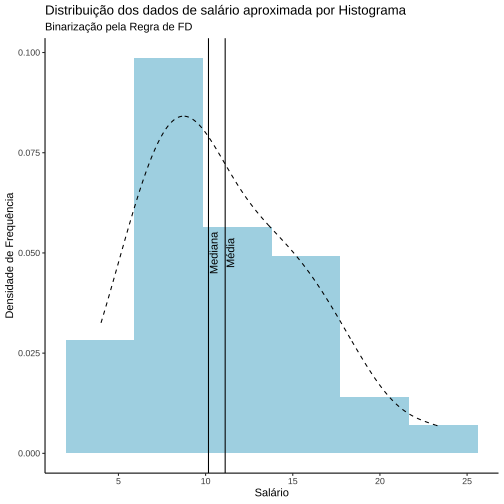
\includegraphics{Antonio-Vieira-dos-Santos-Neto_Estatisticas-para-Cientista-de-Dados_pd_files/figure-latex/analisando salario visualmente com kernel e bin FD -1.pdf}

\begin{Shaded}
\begin{Highlighting}[]
\NormalTok{Bevolucao.roubos.f5.tbl }\SpecialCharTok{\%\textgreater{}\%}\NormalTok{ dplyr}\SpecialCharTok{::}\FunctionTok{select}\NormalTok{(roubo\_transeunte\_sum) }\SpecialCharTok{\%\textgreater{}\%} \FunctionTok{ggplot}\NormalTok{(}\FunctionTok{aes}\NormalTok{(}\AttributeTok{x=}\NormalTok{roubo\_transeunte\_sum))}\SpecialCharTok{+}\FunctionTok{geom\_histogram}\NormalTok{(}\FunctionTok{aes}\NormalTok{(}\AttributeTok{y =} \FunctionTok{after\_stat}\NormalTok{(density)) , }\AttributeTok{binwidth=}\NormalTok{sr, }\AttributeTok{fill =} \StringTok{\textquotesingle{}lightblue\textquotesingle{}}\NormalTok{) }\SpecialCharTok{+} \FunctionTok{xlab}\NormalTok{(}\StringTok{\textquotesingle{}roubo\_transeunte\_sum\textquotesingle{}}\NormalTok{) }\SpecialCharTok{+} \FunctionTok{ylab}\NormalTok{(}\StringTok{\textquotesingle{}Densidade de Frequência\textquotesingle{}}\NormalTok{) }\SpecialCharTok{+} \FunctionTok{labs}\NormalTok{(}\AttributeTok{title =} \StringTok{"Distribuição dos dados de crimes aproximada por Histograma"}\NormalTok{, }\AttributeTok{subtitle =} \StringTok{"Binarização pela Regra de Sturge"}\NormalTok{) }\SpecialCharTok{+} \FunctionTok{geom\_vline}\NormalTok{(}\AttributeTok{xintercept=}\FunctionTok{c}\NormalTok{(}\FunctionTok{median}\NormalTok{(Bevolucao.roubos.f5.tbl}\SpecialCharTok{$}\NormalTok{roubo\_transeunte\_sum), }\FunctionTok{mean}\NormalTok{(Bevolucao.roubos.f5.tbl}\SpecialCharTok{$}\NormalTok{roubo\_transeunte\_sum))) }\SpecialCharTok{+} \FunctionTok{annotate}\NormalTok{(}\StringTok{"text"}\NormalTok{, }\AttributeTok{x=}\FunctionTok{median}\NormalTok{(Bevolucao.roubos.f5.tbl}\SpecialCharTok{$}\NormalTok{roubo\_transeunte\_sum) }\SpecialCharTok{+} \FloatTok{0.3}\NormalTok{, }\AttributeTok{y=}\FloatTok{0.05}\NormalTok{, }\AttributeTok{label=}\StringTok{"Mediana"}\NormalTok{, }\AttributeTok{angle=}\DecValTok{90}\NormalTok{) }\SpecialCharTok{+} \FunctionTok{annotate}\NormalTok{(}\StringTok{"text"}\NormalTok{, }\AttributeTok{x=}\FunctionTok{mean}\NormalTok{(Bevolucao.roubos.f5.tbl}\SpecialCharTok{$}\NormalTok{roubo\_transeunte\_sum) }\SpecialCharTok{+} \FloatTok{0.3}\NormalTok{, }\AttributeTok{y=}\FloatTok{0.05}\NormalTok{, }\AttributeTok{label=}\StringTok{"Média"}\NormalTok{, }\AttributeTok{angle=}\DecValTok{90}\NormalTok{) }\SpecialCharTok{+} \FunctionTok{geom\_density}\NormalTok{(}\AttributeTok{linetype =} \DecValTok{2}\NormalTok{) }\SpecialCharTok{+} \FunctionTok{theme\_classic}\NormalTok{()}
\end{Highlighting}
\end{Shaded}

\begin{verbatim}
## Adding missing grouping variables: `Regiao`, `ano`
\end{verbatim}

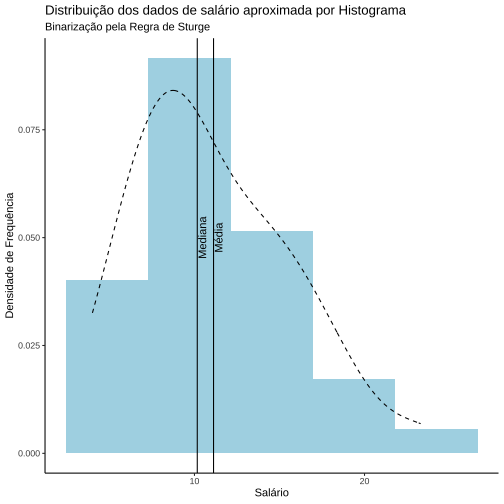
\includegraphics{Antonio-Vieira-dos-Santos-Neto_Estatisticas-para-Cientista-de-Dados_pd_files/figure-latex/analisando salario visualmente com kernel e bin SR -1.pdf}

\begin{itemize}
\tightlist
\item
  CONCLUSÃO :
\end{itemize}

Para as características da base analisada, com uma assimetria acentuada, a regra de FD (Freedman Diaconis), se demonstra mais adequada para a análise.

\hypertarget{analise-inter-variuxe1veis}{%
\paragraph{Analise inter variáveis}\label{analise-inter-variuxe1veis}}

Neste caso farei o filtro para selecionando as localidades que tenham valores para apreensão de drogas (apreensao\_drogas\_sum) que deverá ser comparado com outras 4 variaveis da base.

\#\#\texttt{\{r\ Correlacao\ de\ variaveis\ ,\ echo\ =\ TRUE\}\ \#\#\ kable(cor(Bevolucao.roubos.f5.tbl\ \%\textgreater{}\%\ dplyr::filter(!is.na(apreensao\_drogas\_sum))\ \%\textgreater{}\%\ \#\#\ dplyr::select(apreensao\_drogas\_sum,\ \#\#\ roubo\_transeunte\_sum,roubo\_celular\_sum,roubo\_residencia\_sum)))\ \ \#\#}

\begin{itemize}
\tightlist
\item
  Scatterplot apreensao\_drogas\_sum x roubo\_transeunte\_sum
\end{itemize}

\begin{Shaded}
\begin{Highlighting}[]
\NormalTok{Bevolucao.roubos.f5.tbl }\SpecialCharTok{\%\textgreater{}\%}\NormalTok{ dplyr}\SpecialCharTok{::}\FunctionTok{filter}\NormalTok{(}\SpecialCharTok{!}\FunctionTok{is.na}\NormalTok{(apreensao\_drogas\_sum)) }\SpecialCharTok{\%\textgreater{}\%}\NormalTok{ dplyr}\SpecialCharTok{::}\FunctionTok{select}\NormalTok{(apreensao\_drogas\_sum, roubo\_transeunte\_sum,roubo\_celular\_sum,roubo\_residencia\_sum) }\SpecialCharTok{\%\textgreater{}\%} \FunctionTok{ggplot}\NormalTok{(}\FunctionTok{aes}\NormalTok{(}\AttributeTok{x=}\NormalTok{apreensao\_drogas\_sum, }\AttributeTok{y =}\NormalTok{roubo\_transeunte\_sum)) }\SpecialCharTok{+} \FunctionTok{geom\_point}\NormalTok{() }\SpecialCharTok{+} \FunctionTok{geom\_smooth}\NormalTok{(}\AttributeTok{method =} \StringTok{"lm"}\NormalTok{, }\AttributeTok{se =} \ConstantTok{FALSE}\NormalTok{) }\SpecialCharTok{+} \FunctionTok{theme\_classic}\NormalTok{()}
\end{Highlighting}
\end{Shaded}

\begin{verbatim}
## Adding missing grouping variables: `Regiao`, `ano`
## `geom_smooth()` using formula = 'y ~ x'
\end{verbatim}

\includegraphics{Antonio-Vieira-dos-Santos-Neto_Estatisticas-para-Cientista-de-Dados_pd_files/figure-latex/analisando scatter entre variaveis mais correlacionadas3 -1.pdf}

\begin{itemize}
\tightlist
\item
  Scatterplot apreensao\_drogas\_sum x roubo\_celular\_sum
\end{itemize}

\begin{Shaded}
\begin{Highlighting}[]
\NormalTok{Bevolucao.roubos.f5.tbl }\SpecialCharTok{\%\textgreater{}\%}\NormalTok{ dplyr}\SpecialCharTok{::}\FunctionTok{filter}\NormalTok{(}\SpecialCharTok{!}\FunctionTok{is.na}\NormalTok{(apreensao\_drogas\_sum)) }\SpecialCharTok{\%\textgreater{}\%}\NormalTok{ dplyr}\SpecialCharTok{::}\FunctionTok{select}\NormalTok{(apreensao\_drogas\_sum, roubo\_transeunte\_sum,roubo\_celular\_sum,roubo\_residencia\_sum) }\SpecialCharTok{\%\textgreater{}\%} \FunctionTok{ggplot}\NormalTok{(}\FunctionTok{aes}\NormalTok{(}\AttributeTok{x=}\NormalTok{apreensao\_drogas\_sum, }\AttributeTok{y =}\NormalTok{roubo\_celular\_sum)) }\SpecialCharTok{+} \FunctionTok{geom\_point}\NormalTok{() }\SpecialCharTok{+} \FunctionTok{geom\_smooth}\NormalTok{(}\AttributeTok{method =} \StringTok{"lm"}\NormalTok{, }\AttributeTok{se =} \ConstantTok{FALSE}\NormalTok{) }\SpecialCharTok{+} \FunctionTok{theme\_classic}\NormalTok{()}
\end{Highlighting}
\end{Shaded}

\begin{verbatim}
## Adding missing grouping variables: `Regiao`, `ano`
## `geom_smooth()` using formula = 'y ~ x'
\end{verbatim}

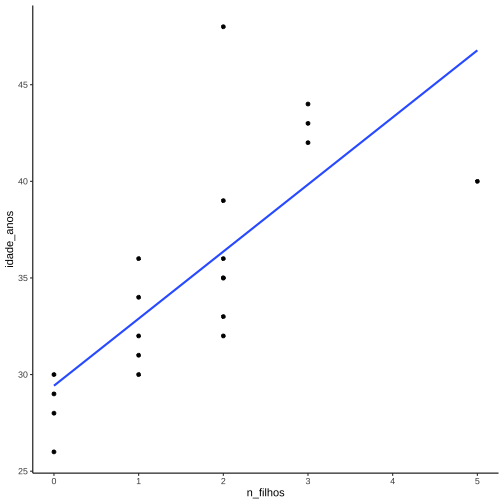
\includegraphics{Antonio-Vieira-dos-Santos-Neto_Estatisticas-para-Cientista-de-Dados_pd_files/figure-latex/analisando scatter entre variaveis mais correlacionadas -1.pdf}

\begin{itemize}
\tightlist
\item
  Scatterplot apreensao\_drogas\_sum x roubo\_residencia\_sum
\end{itemize}

\begin{Shaded}
\begin{Highlighting}[]
\NormalTok{Bevolucao.roubos.f5.tbl }\SpecialCharTok{\%\textgreater{}\%}\NormalTok{ dplyr}\SpecialCharTok{::}\FunctionTok{filter}\NormalTok{(}\SpecialCharTok{!}\FunctionTok{is.na}\NormalTok{(apreensao\_drogas\_sum)) }\SpecialCharTok{\%\textgreater{}\%}\NormalTok{ dplyr}\SpecialCharTok{::}\FunctionTok{select}\NormalTok{(apreensao\_drogas\_sum, roubo\_transeunte\_sum,roubo\_celular\_sum,roubo\_residencia\_sum) }\SpecialCharTok{\%\textgreater{}\%} \FunctionTok{ggplot}\NormalTok{(}\FunctionTok{aes}\NormalTok{(}\AttributeTok{x=}\NormalTok{apreensao\_drogas\_sum, }\AttributeTok{y =}\NormalTok{roubo\_residencia\_sum)) }\SpecialCharTok{+} \FunctionTok{geom\_point}\NormalTok{() }\SpecialCharTok{+} \FunctionTok{geom\_smooth}\NormalTok{(}\AttributeTok{method =} \StringTok{"lm"}\NormalTok{, }\AttributeTok{se =} \ConstantTok{FALSE}\NormalTok{) }\SpecialCharTok{+} \FunctionTok{theme\_classic}\NormalTok{()}
\end{Highlighting}
\end{Shaded}

\begin{verbatim}
## Adding missing grouping variables: `Regiao`, `ano`
## `geom_smooth()` using formula = 'y ~ x'
\end{verbatim}

\includegraphics{Antonio-Vieira-dos-Santos-Neto_Estatisticas-para-Cientista-de-Dados_pd_files/figure-latex/analisando scatter entre variaveis mais correlacionadas2 -1.pdf}

\begin{itemize}
\tightlist
\item
  Criando um grafico de barras, utilizando 2 variaveis
\end{itemize}

\begin{Shaded}
\begin{Highlighting}[]
\FunctionTok{ggplot}\NormalTok{(Bevolucao.roubos.f5.tbl }\SpecialCharTok{\%\textgreater{}\%}\NormalTok{ dplyr}\SpecialCharTok{::}\FunctionTok{filter}\NormalTok{(munic }\SpecialCharTok{==}\StringTok{"Angra dos Reis"}\SpecialCharTok{|}\NormalTok{munic }\SpecialCharTok{==} \StringTok{"Araruama"}\SpecialCharTok{|}\NormalTok{ munic}\SpecialCharTok{==}\StringTok{"Cabo Frio"} \SpecialCharTok{|}\NormalTok{munic}\SpecialCharTok{==}\StringTok{"Cambuci"}\NormalTok{) }\SpecialCharTok{\%\textgreater{}\%}\NormalTok{ dplyr}\SpecialCharTok{::}\FunctionTok{select}\NormalTok{(munic, roubo\_rua\_sum), }\FunctionTok{aes}\NormalTok{(}\AttributeTok{x =}\NormalTok{ munic, }\AttributeTok{y =}\NormalTok{roubo\_rua\_sum)) }\SpecialCharTok{+} \FunctionTok{geom\_bar}\NormalTok{(}\AttributeTok{stat =} \StringTok{"identity"}\NormalTok{)}
\end{Highlighting}
\end{Shaded}

\begin{verbatim}
## Adding missing grouping variables: `Regiao`, `ano`
\end{verbatim}

\includegraphics{Antonio-Vieira-dos-Santos-Neto_Estatisticas-para-Cientista-de-Dados_pd_files/figure-latex/grafico de barras-1.pdf}

\end{document}
